\section{Results II: Outcome Memorization and the Candidate Budget}
\label{sec:results2}

\textbf{The phenomenon.}
\label{sec:phenomenon}
Regression reaches a memorization index of $0.99$ on A2-div: it learns which mode every training context took. \imlewm{} with $m{=}4$ climbs to $0.75$ while its held-out coverage falls from $0.77$ at 4k steps to $0.46$ at 12k steps (Figure~\ref{fig:curves}, Appendix~\ref{app:more}); on held-out contexts its index stays at chance, so this is memorization of the realized outcome of each training context, keyed on the context's appearance, rather than a failure to generalize. Training the $m{=}4$ model twice as long, or making it $2.7\times$ larger, raises the index further and lowers coverage (Appendix~\ref{app:more}), so the collapse is not under-training. On A2-fix, where the identifying key is absent, the same $m{=}4$ recipe does not memorize (index $0.26$) and covers $0.97$ of the modes (Table~\ref{tab:es}, Appendix~\ref{app:es}), and with $m{=}16$ the index stays at $0.29$ even when training runs $1.5\times$ longer. The budget, not the recipe, determines whether the model memorizes.

\begin{figure}[t]
\centering
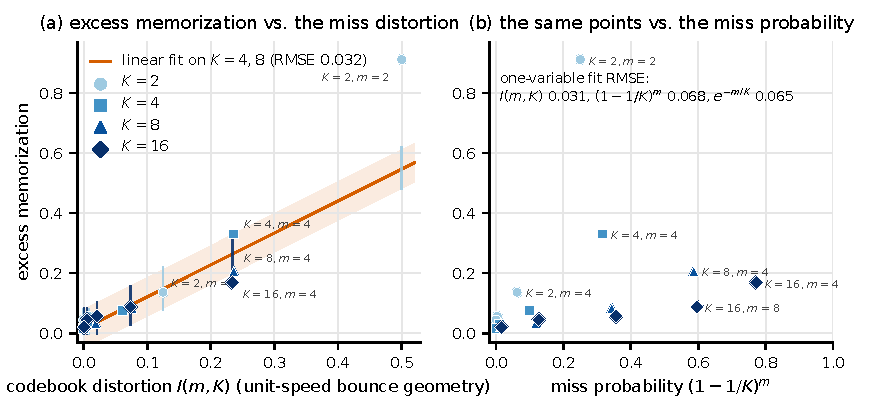
\includegraphics[width=\linewidth]{fig_memo_collapse.pdf}
\caption{Excess memorization on A2-div at 8k steps (two seeds) for $K\in\{2,4,8,16\}$, $m\in\{2,\dots,64\}$. (a) Against the codebook distortion $I(m,K)$ of Equation~\ref{eq:I} (exact for the bounce geometry); line and band: the linear fit on the $K{=}4,8$ points ($\pm2$ RMSE) from which the $K{=}2,16$ predictions were recorded before those runs; vertical bars: the recorded intervals. (b) The same points against the miss probability $(1-1/K)^m$ used by \citet{gladstone2026xm} and \citet{bennett2026freedom}: no collapse.}
\label{fig:collapse}
\end{figure}

\textbf{Excess memorization collapses onto $I(m,K)$.}
\label{sec:collapse}
Proposition~\ref{prop:memo} says that the incentive is the codebook's miss distortion. We trained \imlewm{} for $K \in \{4, 8\}$ and $m \in \{4, 8, 16, 32\}$ (two seeds, 8k steps), fitted excess memorization as a linear function of $I(m,K)$ on those eight points ($0.015 + 1.06\,I$, RMSE $0.032$), recorded predictions with $\pm2$ RMSE intervals for nine runs at $K \in \{2, 16\}$, and only then trained those runs. Seven of the nine fell inside their interval (Figure~\ref{fig:collapse}a; Table~\ref{tab:grid}, Appendix~\ref{app:more}). The two misses lie at the ends of the range and in the directions we had noted as risks: at $K{=}2$, $m{=}2$ ($I = 0.50$, outside the fitted range) memorization is stronger than the linear extrapolation ($0.96$ vs.\ $0.77$), and at $K{=}16$, $m{=}4$ it is weaker ($0.22$ vs.\ $0.31$), consistent with a capacity effect, since storing one of 16 outcomes per context costs $\log_2 16$ bits. The alternative hypothesis, that the budget should scale with the number of modes, is rejected: at a fixed $m{=}8$ the excess memorization is $0.075$, $0.083$ and $0.087$ for $K = 4$, $8$ and $16$, as the nearly equal values of $I(8, K)$ on this geometry predict, whereas at a fixed ratio $m/K = 1$ it ranges from $0.91$ to $0.06$; a one-variable linear fit on all points except the extrapolated one has an RMSE of $0.031$ in $I(m,K)$, against $0.068$ in $(1-1/K)^m$ and $0.065$ in $e^{-m/K}$ (Figure~\ref{fig:collapse}b). The linear relation holds for $I \lesssim 0.25$ and saturates above it. The practical rule is that $m$ must make $I(m)$ small relative to the mode spacing on the outcome manifold; here $m = 16$--$32$ brings the excess memorization below $0.05$ for every $K$.

\begin{figure}[t]
\centering
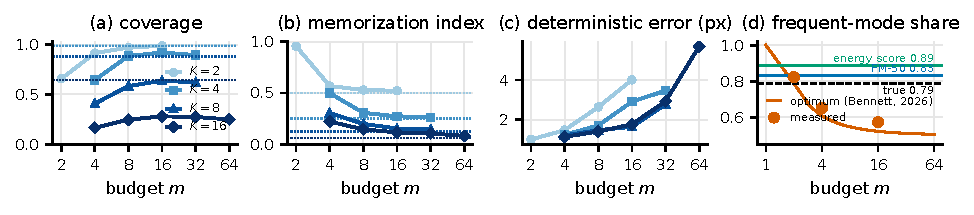
\includegraphics[width=\linewidth]{fig_m_knob_main.pdf}
\caption{What the budget controls (A2-div, 8k steps, two seeds; shade = $K$). (a) Coverage peaks at $m{=}16$ (dotted: ideal sampler) while (b) the memorization index approaches chance (dotted). (c) The deterministic-transition error grows with $m$; training time grows about threefold from $m{=}4$ to $m{=}32$, inference cost not at all (all panels in Appendix~\ref{app:more}). (d) With unequal mode probabilities ($K{=}2$, $p{=}0.79$) the frequent-mode share of \imlewm{} samples falls with $m$ along the optimum of \citet{bennett2026freedom}; FM-50 is calibrated and the energy score over-represents the frequent mode (Section~\ref{sec:flatten}).}
\label{fig:knob}
\end{figure}

\textbf{Countermeasures and the cost of $m$.}
\label{sec:counter}
Raising $m$ is the cleanest way to remove the incentive (Table~\ref{tab:counter}, Appendix~\ref{app:more}): RS-IMLE rejection of candidates already within $\epsilon$ of the target \citep{vashist2024rsimle} changes nothing at $m{=}4$, and Gaussian noise on the context tokens ($\sigma = 1.0$) removes the key and the memorization (index $0.27$) but blurs information the prediction needs (coverage $0.74$, precision $0.61$, deterministic-transition error $1.92$\,px). Figure~\ref{fig:knob} shows the costs of $m$ itself: at 8k steps the deterministic-transition error grows from $1.2$\,px at $m{=}4$ to $2.8$--$3.5$\,px at $m{=}32$ (less with longer training), training time grows about threefold, and coverage and precision saturate at $m{=}16$. The recipe is otherwise insensitive: replacing Geman--McClure by $\ell_2$, or the 256-dimensional noise by a 64-dimensional one, changes coverage and the index by at most $0.01$ (Appendix~\ref{app:impl}).

\textbf{A strictly proper score memorizes regardless of $m$.}
\label{sec:es}
Proposition~\ref{prop:es} predicts that an energy-score generator memorizes in non-repeating contexts at every budget. Trained on A2-div with the \imlewm{} generator unchanged, it does (Table~\ref{tab:a2}; Table~\ref{tab:es} in Appendix~\ref{app:es}): the index reaches $0.87$ at $m{=}8$ and $0.97$ at $m{=}16$ (chance $0.25$); its held-out coverage peaks at $0.50$ near 6k steps and then falls to $0.36$ as the index rises; and a larger $m$ makes it memorize \emph{faster} (index $0.84$--$0.87$ at 8k steps for the two $m{=}16$ seeds, against $0.51$--$0.72$ for the three $m{=}8$ seeds), as expected if $m$ only reduces the gradient variance towards the same minimizer. A per-token energy score, a common choice for continuous tokens, memorizes as well (index $0.97$, coverage $0.22$). The ordering across objectives follows the relative incentives of Section~\ref{sec:theory_es} (regression $0.99$, energy score $0.87$--$0.97$, \nom{} $0.75$ at $m{=}4$ and $0.29$ at $m{=}16$), and with unequal mode probabilities the energy score has no calibration advantage either (frequent-mode share $0.89$ against a true share of $0.79$, coverage $0.58$; Figure~\ref{fig:knob}d).


Memorization requires an incentive, an identifying key and enough revisits of each context. A toy two-branch problem after \citet{makabe2026esp} with a 16-dimensional nuisance ``appearance'' vector in the context reproduces their result when every training context is fresh (the energy score places $0.94$ of its samples on a mode, \nom{} $0.92$; they report $0.962$ and $0.919$), but with $1{,}024$ fixed training contexts the energy score memorizes completely (index $0.999$) and covers both modes on almost no new context, whereas \nom{} stays at $0.51$ and covers $0.99$--$1.00$; removing the appearance vector, or using $16{,}384$ or more contexts, removes the energy score's memorization as well (Appendix~\ref{app:es}). Both conditions transfer to the full environment: the five predictions recorded before the A2-fix and per-token runs (the energy score does not memorize on A2-fix but still trails \imlewm{} in coverage and precision; the per-token variant memorizes on A2-div) all held, and on A2-fix the coverage gap shrinks from $0.57$ to $0.04$ while a precision gap of $0.14$ remains. A second cause is spread off the manifold. On Bouncing Shapes, where nothing can be memorized, the energy score still trails \imlewm{} and regression (F1 $8.9$ vs.\ $7.2$ and $8.1$\,px); its error rises to $33.8$\,px under FlowWM's clean heatmap readout and falls back to $11.7$\,px under a readout trained with feature noise $0.5$, whereas \imlewm{} and regression move by less than $0.5$\,px; and on A2-div its token-space spread exceeds that of \imlewm{} while its readout spread is less than half (Appendix~\ref{app:readout}). The diversity is spent in directions that readouts do not see, as the direction-insensitivity argument suggests. The conclusion is conditional: with fresh contexts or without an identifying feature the energy score is competitive, but in non-repeating contexts with identifying appearance, the property that \citet{makabe2026esp} list as a defect of the hard minimum, namely that it is not strictly proper for finite $m$, is precisely what lets \nom{} escape memorization by raising $m$.
